\chapter{The physics behind sailboats}
%In \cite{philpott1993yacht} and \cite{larsonprinciples} agree that the essential or basic principles about the mechanics of sailing have been know since 1950's, and in 1979 Marchaj  published a book, \cite{marchaj1979aero} to compile and review the available knowledge about sailing and add information which is still being used for yacht design, like coefficients and other calculations. Because  sailboats move through 2  different fluids it is important to know how the elements are named and which words are related with specific maneuvers.  These simple concepts, will help you to understand how the equilibrium is generated in the static and steady  state, what elements interacts on it and how the balance is conserved when the sailboat moves from one point to another. 
Sailing boats are propelled mainly by wind, however they displace through the water; in other words, sailboats move through 2 different fluids: water and wind. The mechanics of sailing have been know since 1950's.  Marchaj in 1979 review them and add information which is still being used for yacht design \cite{marchajaereo1979}.\par 

This chapter is focus on the motion of the sailboats, what are physics behind, which forces interact in equilibrium and during motion. How the athlete takes part of this model and what other consideration are required to set-up the equations of motion. Since sailboats are govern by similar equations some adjustments are required to differentiate between yachts and lasers this adjustments are explained at the end of the chapter. The equations of motion facilitate the identification of variables that can be use as a parameter to model the trajectory as well as to identify its limitations. These considerations are required to optimize the trajectory and obtain the minimal time path. \par
\section{Interaction between the sailboat, water and air}
The origin of the forces and momentum depends on the interaction of the elements of the sailboat with the 2 mediums, water and air. Some of this forces are clear, like the forces acting above the water surface which are produced by the wind and the interaction of it with the sails. These forces have to be balanced by the forces beneath the same surface; in this case, the water interacts with the hull, rudder and keel. Therefore by adjusting the sail and the rudder, the only movable elements, the sailboat can hold a steady course.\par

Philpott explains how different elements, parts of the sailboat, interact with the surroundings and how they are used to control and attain the equilibrium during motion. Figure \ref{sailboat_terms} shows the most common elements and where are they located. Some of those elements can be manipulated by the seamanship, which means that the variables concerned can be controlled and therefore they are know as control variables \cite{philpott1993yacht}. \par
%In addition, 
%The main elements of the sailboat, including wind, currents and waves were grouped in 3 categories that affect the equilibrium in a different way \cite{philpott1993yacht}.
 %\begin{enumerate} \label{factorphil}
% \setlength \itemsep{0em}
% \item Environmental factors; such as wind and current intensity and direction,
% \item Design factor, dimensions that characterize the type of boat. 
 %\item Control variables, variables affecting by the seamanship
 %\end{enumerate}
 \begin{figure}%[ht]
\centering
  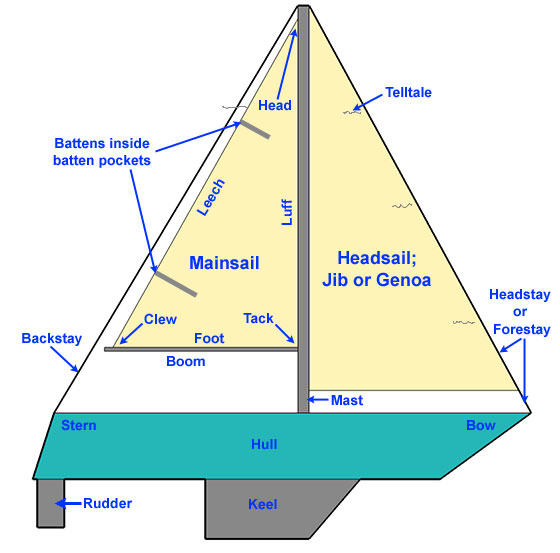
\includegraphics[width=0.4\linewidth]{sailboat_terms.jpg}
 \caption{Common sailboat terms \cite{sailboat_terms}. }
\label{sailboat_terms}
\end{figure}
In order to steer a boat the seamanship has to control the angle of the rudder, this interacts directly with the current, the direction obtained is called \textit{heading} and these two, rudder and current, generate forces that influence the boat to \textit{yaw}. \par
Due to the wind direction, mainly, the boat slip sideways and this effect is know as \textit{leeway}. The difference in course comparing with the heading is expressed as \textit{leeway angle ($\lambda$)}. %, which can be see in the figure \ref{forces_m} \textit{C}.
The sails adjustment is known as trim; when the trim reduce the area of the sail then the seaman is \textit{reefing}, most of the time this term refers when the size of the sails is changing.  Reefing under sail allows the seamanship to control the wind intensity. \par
The wind over the sails, generates a force and an angle called \textit{heel angle}; which can be see in the figure \ref{forces_m} \textit{B}, this decrease the driving force. Under those circumstances, a moment is generated and to neutralize it, the seamanship generates a \textit{righting moment} (\textit{ $M_{R}$}) by standing on the windward side of the boat to produce it\cite{philpott1993yacht}. %A graphical representation of the interaction of these forces is  found in \ref{forces_m}.
As a result of these forces, the velocity could be optimal or not. \cite{larsonprinciples} relates the factors and forces proposed in\cite{philpott1993yacht} in terms of forces and resistances, indicating how the dynamics of each of the mediums, water and air, interact to keep the balance (and be capable to maximize the boat's speed). Therefore, the forces and resistances are related as showed below: \par 
\begin{itemize}  \label{milgramforces}
 \setlength \itemsep{0em}
\item Aerodynamic driving forces = Hydrodynamic resistance;
\item Aerodynamic side force = Hydrodynamic side force;
\item Aerodynamic heeling moment=Hydrodynamic (static) righting moment.
\end{itemize}
An important assumption made by  \cite{philpott1993yacht} and \cite{larsonprinciples} to keep the analysis of the boat in 2 dimensions is that vertical forces are in balance always, same as the pitching moment; Figure \ref{forces_m} \textbf{c} shows the only forces that acts when this assumption is made; additionally 2 angles are shown, one of then refers to the wind.\par

\section{Planes of motion}
Sailing boats are considered rigid bodies that can move in a three dimensional space; figure \ref{DOF} shows the 6 fundamental types of motion or degrees of freedom (DOF)  with the names and axis where they are referred: three translations and three rotations. \par 
It also shows the water surface which is represented by the plane \textit{XY} and the orientation of the sailboat shows the positive direction of the three axes which follow the right-hand orthogonal system. Thus, \textit{X} axis is positive in the direction of the motion, \textit{Y} is positive to port or left side of the sailboat and \textit{Z} is positive upwards. In the case of the \textit{Y} axis the negative direction or right side of the sailboat is know as starboard.  Besides, for future references, the speed of the boat is along the \textit{X} axis. These six DOF correspond to three forces and three moments which are going to explain in the next section. \par 
\begin{figure} %[ht]
\centering
  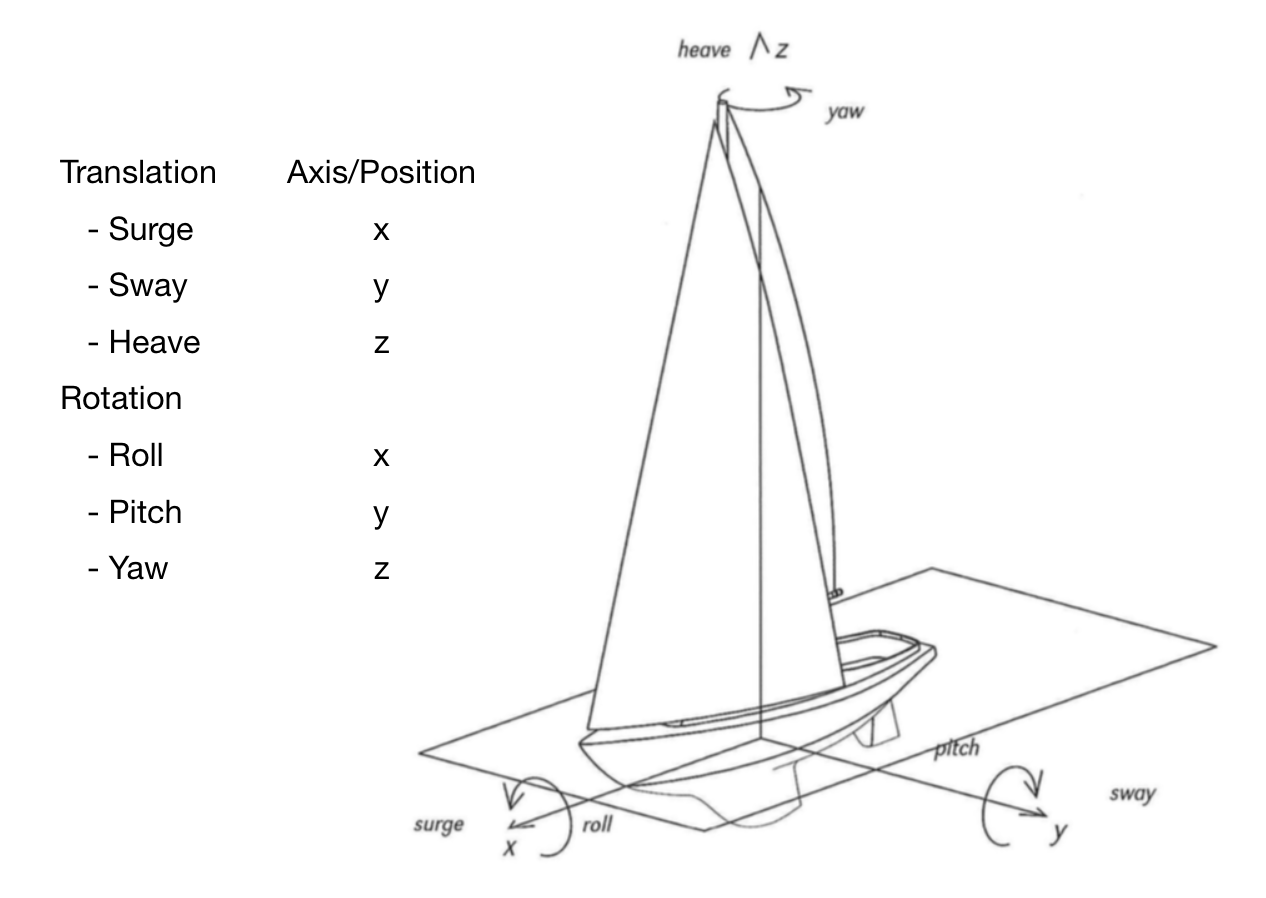
\includegraphics[width=0.7\linewidth]{dof_foss_modif.png}
 \caption{Degrees of freedom of a boat, clockwise reference system xyz \cite{fossati2009aero}. }
\label{DOF}
\end{figure}

Because the sail boat interact between two fluids not only they generate forces but also resistances in both mediums. It is important to know how the elements are named and which words are related with specific axis.  These simple concepts are useful to understand how the equilibrium is generated in the static condition, what elements interacts on it and how it is conserved when the sailboat moves from one point to another. \par 

\section{Hydrodynamic and Aerodynamic Forces and Momentum} \label{section:forces_moment}
The static and dynamic balance of any type of boat is based on Newton's second law. However, when the boat moves, a dynamic situation, it is the winds' velocity that leads this equilibrium. Because the sail boat interact between two fluids they not only  generate forces but also resistances.
The next equations basically show that the total aerodynamic force ($F_{A}$) is equal and opposite to the total hydrodynamic force ($F_{H_{TOT}}$). \par

\subsection{Wind and the Velocity Triangle}
In sailing, the wind is characterized by its speed and direction and it is defined as \textit{true wind ($_{tw}$)} and \textit{true wind angle ($\beta_{t}$)}.  Because it also interacts with the water surface, in some cases its intensity depends on the height where it was measured, to know its value at different height it is estimated by the equation \ref{eq:wind_h}. According \cite{claughton1998sailing} the exponent $\kappa$ has a value between 1/7 and 1/14; and the reference height for measurements is 10m above the water surface. \par 
\begin{equation} \label{eq:wind_h}
    V_{tw}(Z)=V_{tw}(Z_{ref}) \cdot \bigg( \frac{Z}{Z_{ref}} \bigg)^\kappa
\end{equation}

The steady motion of the sailboat not only depends on the balance of forces but also on the relation between velocities, boat and wind, mainly. This interaction is represented by the velocity triangle shown in figure \ref{vel_triangle}. The triangle introduce the apparent wind velocity ($V_{aw}$) and angle ($\beta_{a}$).\par 
\begin{figure}[ht]
\centering
  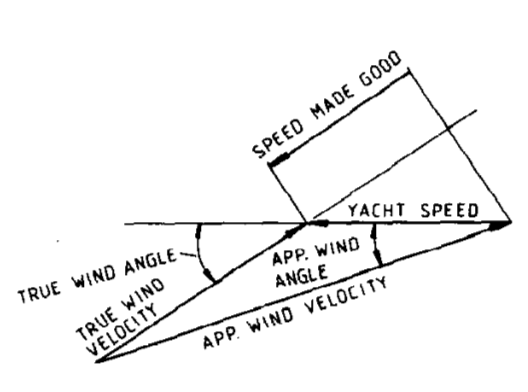
\includegraphics[width=0.65\linewidth]{Larsson_triang_vel.png}
 \caption{Velocity triangle  \cite{larsonprinciples}. }
\label{vel_triangle}
\end{figure}
The $V_{aw}$ and $\beta_{a}$ result from the vector summation of the true wind ($V_{tw}$) and sailboat ($V_{boat}$) velocities; to estimate them it uses the heel angle ($\Theta$), equations \ref{eq:app_angle} and \ref{eq:app_angle} show how to calculate them. These equations include the heel angle because $V_{aw}$ are used to calculate some sail force coefficients which are specified at center of effort (\textit{CE}),its location is about 40\% at the mast height. The $\beta_{a}$ incorporated the leeway angle ($\lambda$), which value is usually less than 6\degree \cite{philpott1993yacht},\cite{claughton1998sailing}. \par
\begin{equation} \label{eq:app_angle}
    \beta_{a}=tan^{-1} \bigg( \frac{ V_{tw} sin \beta_{t} cos \Theta }{ V_{tw} cos \beta_{t} + V_{boat}} \bigg)
\end{equation}
\newline
\begin{equation} \label{eq:ap_vel}
    V_{aw}=  \sqrt{ (V_{tw} sin \beta_{t} cos \Theta)^2 + (V_{tw} cos \beta_{t} + V_{boat})^2}
\end{equation}
\subsection {Equilibrium Equations} \label{section_equil_equat}
In static condition, the equilibrium is reach when the summation of all the forces and momentum equals zero. In figure \ref{forces_m} these forces are located according the planes where they act, the names of them and the fluid that drives them. In addition to the forces and momentum, there are 4 angles to consider. Another observation is how the position and weight of the athlete is incorporated in the equilibrium equations. \par 

The equations of force(\textit{F}) by plane in equilibrium are:
\begin{equation}\label{eq:force_x}
    \text{(Surge, x  \space axis)  \space} F_{R}=R \\
\end{equation}
\begin{equation}\label{eq:force_y}
    \text{(Sway, y\space axis) \space } \space F_{H,lat}=F_{S,lat}\\
\end{equation}
\begin{equation}\label{eq:force_z}
    \text{(Heave, z\space axis)  } \space F_{V}=F_{VW}
\end{equation}
And the those for the momentum (\textit{M}) in equilibrium are:
\begin{equation}\label{eq:m_x}
    \text{(Roll, x  \space axis) \space } M_{R}=M_{H} \\
\end{equation}
\begin{equation}\label{eq:m_y}
    \text{(Pitch, y \space axis)  } \space M_{PA}=F_{PW}\\
\end{equation}
\begin{equation}\label{eq:m_z}
    \text{(Yaw, z \space axis)  } \space M_{YW}=M_{YL}
\end{equation}

 \begin{figure}[ht]
\centering
  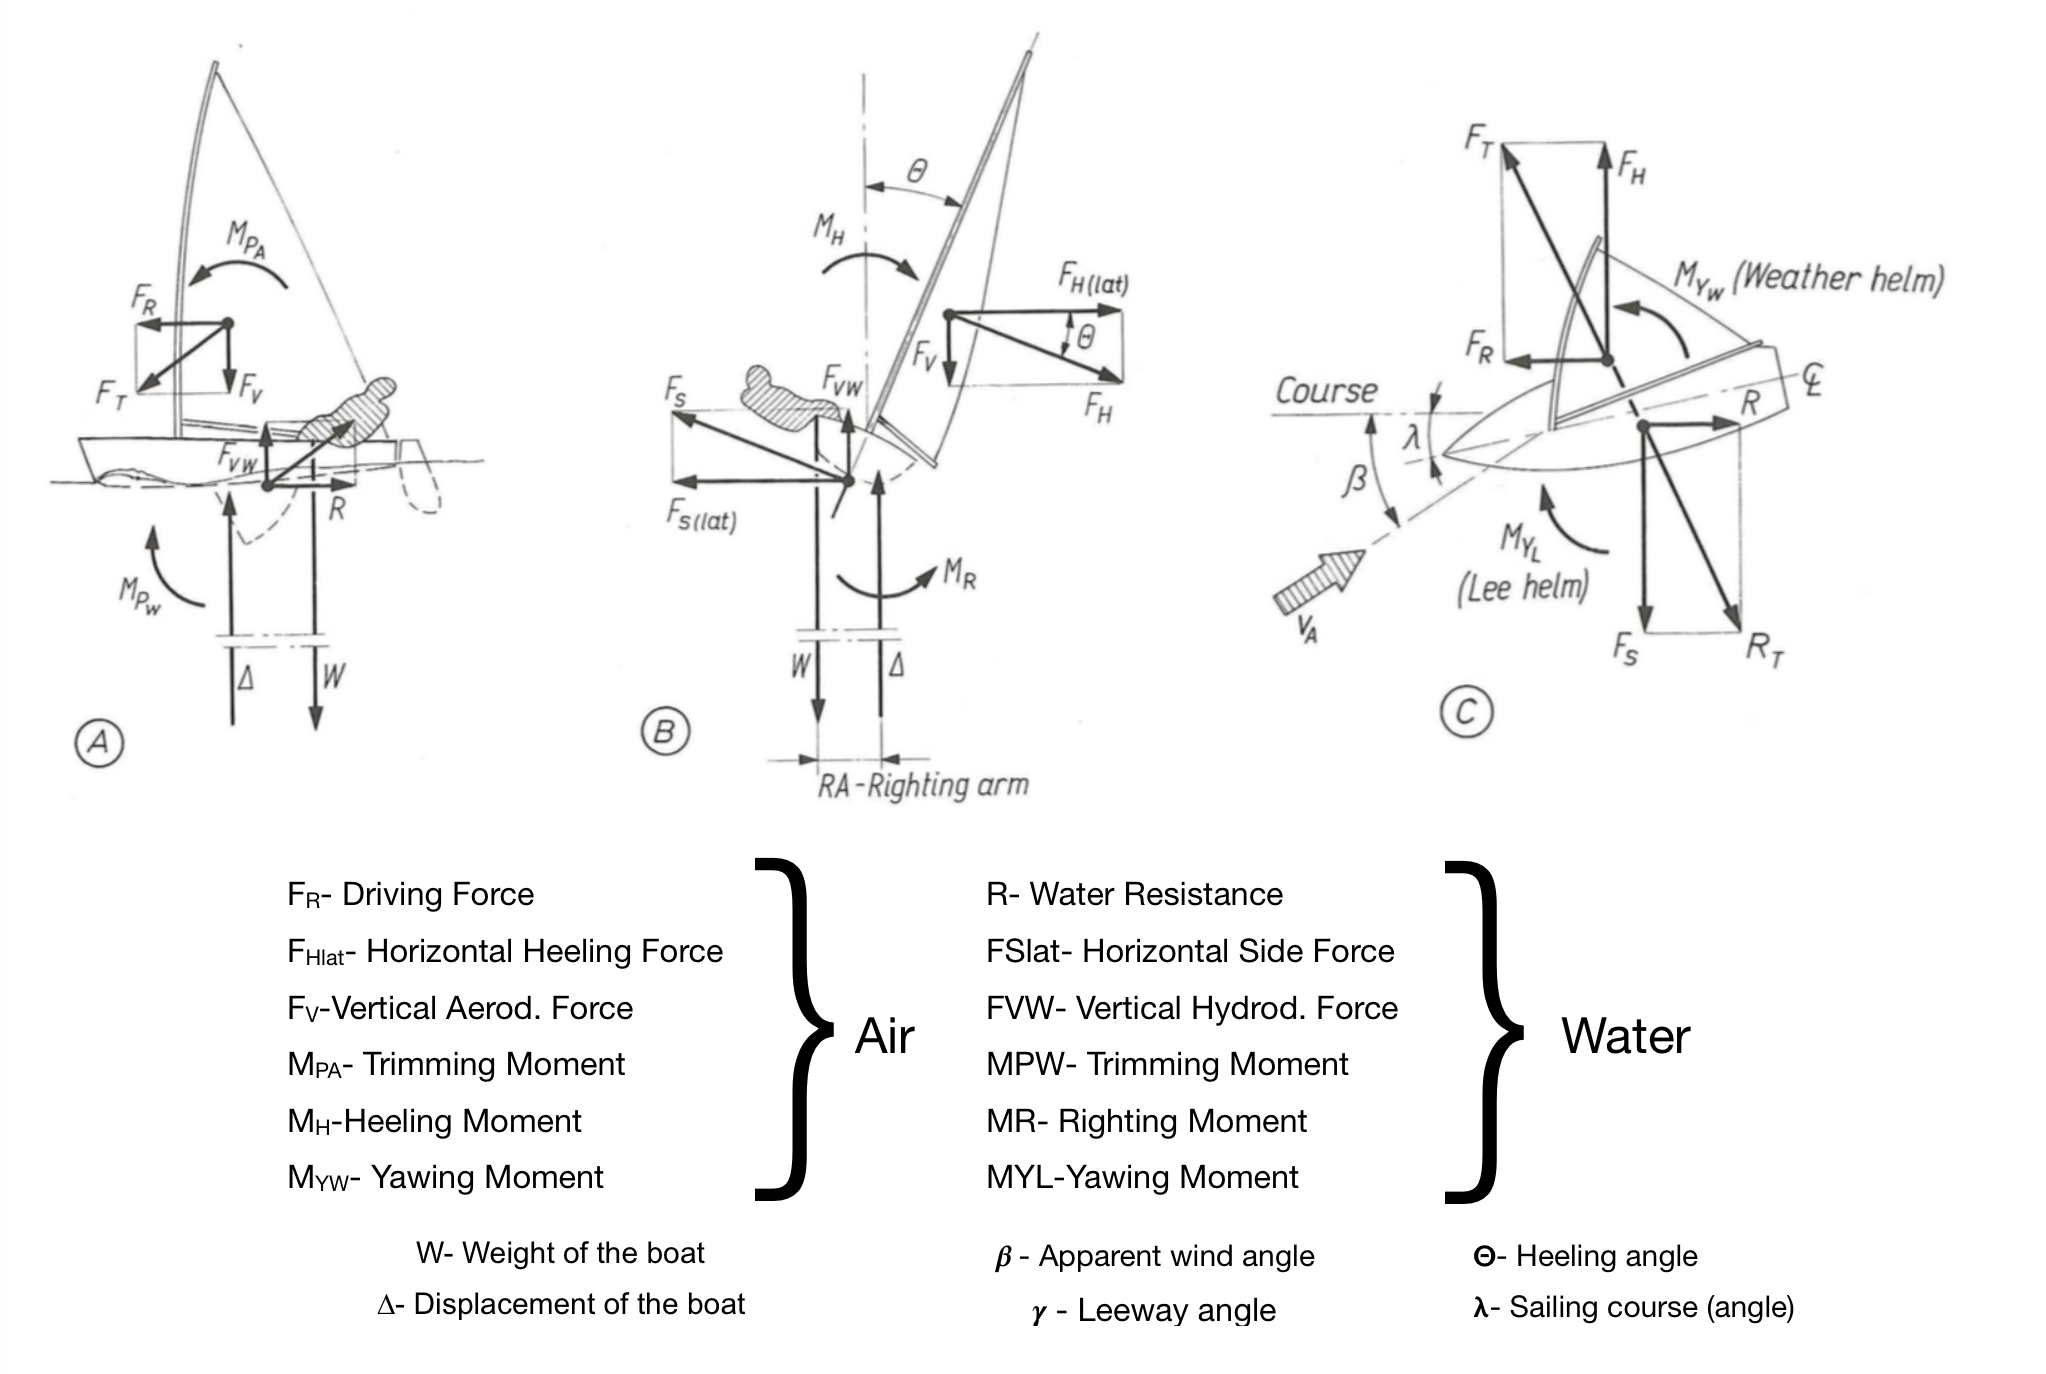
\includegraphics[width=.97\linewidth]{marchaj_forces.png}
 \caption{Equilibrium of forces and moments in steady-state sailing condition \cite{marchajaereo1979} }
\label{forces_m}
\end{figure}

\subsection{Aerodynamic Forces and Resistances}
The force that drives motion of the sailboat is the driving force($F_{R}$); figure \ref{forces_m} \textit{B} shows the force that causes the drift (heel) of the sailboat is the heeling force ($F_{H}$). The motion of the sailboat happens when $F_{R}$ beat the hull resistance (\textit{R}); while in the \textit{ZY} plane the balance of the forces happens when $F_{H}$ equals the hydrodynamic side force ($F_{S}$), which is produced by the effect of the water over the hull. Then:\par 

( Because $F_{A}$ result from $F_{R}$, parallel to the \textit{apparent wind} direction and $F_{H}$ perpendicular to $F_{R}$. Under balance the variables related to them are:)
\begin{multline}
\\
F_{A}=F_{R}(\parallel V_{aw}) + F_{H}(\bot F_{R} )\\
F_{R}=F_{R}(V_{aw},\beta_{a}, \Theta) \\
F_{H}=F_{R}(V_{aw},\beta_{a}, \Theta) \\
F_{S}=F_{S}(V_{boat},\lambda, \Theta) \\
R=R(V_{boat},\lambda, \Theta)\\  
\end{multline}
\\
%th they depend on the $V_{aw}$ and $\beta_{a}$; while $F_{S}$ and \textit{R} depend on $V_{boat}$ and $\lambda$. 
Due to the dependency on velocities,$F_{R}$ and $F_{H}$ generate drag (\textit{D}) and lift (\textit{L}) forces acting normal to the centre plane of the hull and mast and they are integrated in to the forces, according to \cite{philpott1993yacht} and \cite{claughton1998sailing} as: \par 
\begin{equation} \label{eq:Fr_LD}
    F_{R}=L sin \beta_{a} - D cos \beta_{a}
\end{equation}
\begin{equation} \label{eq:Fh_LD}
    F_{H}=(L cos \beta_{a} + D sin \beta_{a}) cos\Theta
\end{equation}
\\ \textit{D} and \textit{L} depends not only depends on  the sail area (\textit{A}),$V_{aw}$, fluid density ($\rho$) but also on coefficients which depends on the trim and flatness of the sail \cite{philpott1993yacht}, \cite{carrico17symp}, \cite{day2017performance}; these last, are under the control of the seamanship. \textit{D} and \textit{L}  are expressed in those terms as follow: \par
\begin{equation} \label{eq:Lift}
  L=qAC_{t}  
\end{equation}
\begin{equation} \label{eq:Draf}
    D=qAC_{d}  
\end{equation}
\begin{equation} \label{eq:dynamic_press}
    q=\frac{1}{2}\rho V_{aw}^2
\end{equation}
\begin{equation} \label{eq:Cd}
    C_{d}=C_{d}(\beta_{a},trim, flatness)
\end{equation}
\begin{equation} \label{eq:Ct}
    C_{t}=C_{t}(\beta_{a},trim, flatness)
\end{equation}
$C_{d}$ and $C_{t}$ values are obtained from tables or graphics and their range is over (0,1), later on this is going to be explain in detail. 
\subsection{Hydrodynamic Forces and Resistances}
$F_{H}$ generates a force below the water surface, which us know as horizontal side force $F_{Slat}$ and it is determined as follow: \par
\begin{equation}
    F_{Slat}= F_{H}cos \Theta
\end{equation}

\subsection{Momentum at the sailboat model}
Because $F_{A}$ is apply at \textit{CE} and $F_{H_Tot}$ at the center of lateral resistance (\textit{CLR}). The moments generated over the sailboat depends on these 4 variables. For example \textit{righting moment M_{R}}, figure \ref{forces_m} \textit{B} is counterbalanced as next: 
\begin{equation}\label{eq:right_mom}
    M_{R}=F_{H}(CE-CLR)_{z}=W \cdot RA
\end{equation}
where:\par
\begin{itemize}
    \item $(CE-CLR)_{z}$ is the heeling arm or the vertical distance between \textit{CE} and \textit{CLR} when $F_{H}$ is perpendicular to it.
    \item W = weight of the boat.
    \item RA = Righting arm or the horizontal distance between the \textit{W} and the \textit{Z} axis.
\end{itemize}
The \textit{yaw moment} $(M_{Y})$ depends most of time, on the rudder angle since it can shifts the \textit{CLR}, another form to change this distance is by trimming which change the area of the sail and therefore the \textit{CE} shifts its location.\par 
The \textit{trimming moment} ($M_{P}$) arise from gravity (\textit{g}) and buoyancy forces, the displacement of the boat (\textit{$\Delta$}) is related with $V_{boat}$ ; for example, at high velocities the lift forces are added to the buoyancy forces at the front sections.\par 
%Becuase $F_{A}$ and of the drag (\textit{D}) and lift (\textit{L}) forces generated by the wind on the sail, more specific the \textit{apparent wind}. (\textit{D}) is at the same direction as the \textit{apparent wind} while (\textit{L}) is perpendicular to (\textit{D}). \par 
In rough water, however the pitching motion reduces the speed and it is compensated by both mediums, the aerodynamic and hydrodynamic forces.\par % Another consideration refers to the wind, the force it generates over the sails is applied at  the center of effort on them which is assumed to be located at 40\% of the mast height \cite{philpott1993yacht}. \par 

%while in a dynamic situation, as when the boats moves, it is the velocity that leads this equilibrium.
\section{Velocity Prediction Polar}
To determine the sailboat velocity between the wind direction and its course, that can be reach under different environmental conditions(wind angle and magnitude), scientist developed in 1979 a velocity prediction program that is plotted in a polar diagram (\textit{VPP}). This program according  \cite{larsonprinciples}, use the equations for static equilibrium and information about the hydrodynamic, aerodynamic and stability properties of the sailboat.  The solution is given by  the forces mentioned in \ref{milgramforces} and the apparent wind velocity and direction. By using the VPP not only the maximum sailboat speed can be obtained and the direction that should be follow but also the angles that should be avoid to stay away from the irons\cite{yang2011control}. These angles range make a zone that is described as the no-go zone.\par 

Because VPP plots are symmetric only half of them are usually represented as shown in the figure \ref {typ_vpp}. The polar diagram indicates the boat speeds by the concentric half circles, the wind speed are the lines that form a half heart shape; the intersection of these lines with straight lines, which indicated the directions, indicates the maximum velocity that a sailboat can attain. The figure \ref{no_go_zone} is the full representation of the VPP and it shows where the no-go zone is located, this zone correspond to the concave curve of the true wind speed.\par 

\begin{figure} %[ht]
  \centering
  \subfloat[VPP plot for true wind angles from 0 \degree to 180\degree and true wind speeds from 4 to 10 m/s (7.77-19.44 kn) \cite{larsonprinciples}.]{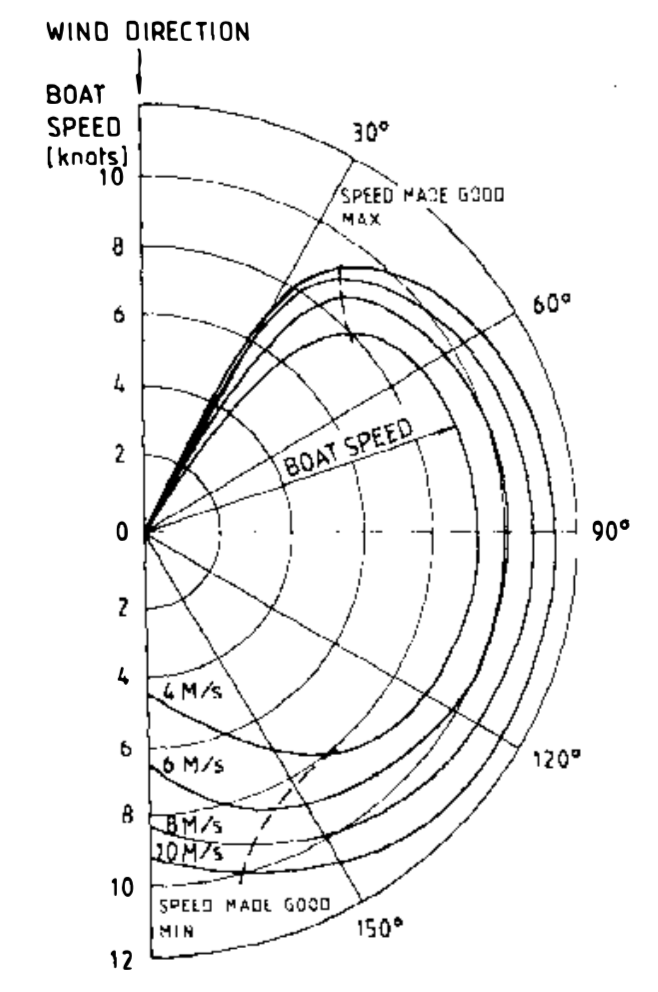
\includegraphics[width=0.37\textwidth]{vppLarsson1990.png}\label{typ_vpp}}
  \hfill
  \subfloat[Polar Curve of the Propulsion System \cite{yang2011control}(Full VPP representation).]{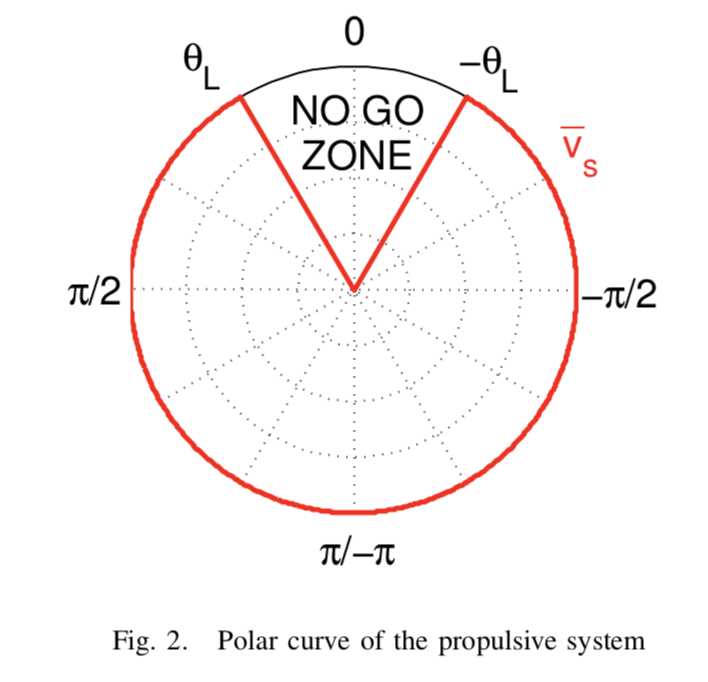
\includegraphics[width=0.5\textwidth]{no-go_zone_yang.png}\label{no_go_zone}}
  \caption{VPP diagram}
\label{vpp_diag} 
\end{figure}

The wind, current and boat velocities interaction is represented with the velocity triangle.  Figure \ref{vel_triangle}, shows the relation between wind and boat (yacht) velocities and the additional resulting velocities; the apparent wind velocity ($V_{aw}$) and speed made good,  also know as velocity made good (vector notation). The figure also shows how the true and apparent wind angle are made. It is important to explain that the velocity of the current is considered in the boat's velocity, equation \ref{eq_vel}; where \textit{tw} is the true wind velocity, \textit{b} means respect to the boat and \textit{c} is the current velocity, $\alpha$ is the sail angle and \textit{V} is the velocity vector. \par 

The velocity made good \textit{(VMG)} provides useful information to understand where the sailboat is on the space and how is its motion \cite{larsonprinciples}. Therefore, this triangle have to be considered for any type of analysis.\par 
%% Include equations here 
\begin{equation}
\label{eq_vel}
\begin{aligned}
V_{aw} & = V_{tw,b} - V_{c,b} - V_{boat}
\end{aligned}
\end {equation}

\begin{equation}
\label{eq:VMG}
\begin{aligned}
VMG &=  \mid V_{boat} cos \alpha  \mid 
\end{aligned}
\end {equation}

$V_{aw}$ and its direction $( \alpha_{aw})$ are highly important because it is the velocity perceived by the moving sailboat and its is given by the difference between the wind and the boat; if the boat is moving in the same direction as the wind then the apparent velocity increase. \par 
%% If height exceed width, then the effective sail area is A=pi h/4. The area of the air used in our calculations depends on the height of the sail, this is explained in the prandt and . The force of the boat is given by  Fboat= Fwind cos (a sail-app wind) cos (avw- sail-app wind). If the boat is in downwind condition veq=wind vel/( 1+ (beta)^0.5 ) and beta = drag factor / (density air * Area sail)

\section{Equations of Motion}
The motion of the boat from one point to another occurs in the XY plane. In the previous sections the different components like forces generated by the wind or water were explained and how the seamanship or athlete compensate these forces by interacting with sailboat via sail or rudder mainly. On section \ref{section:forces_moment} is was explained the interaction of the forces to attained the equilibrium also it was mentioned that the  pitching moment and sway forces (vertical forces) are always in equilibrium, which means that heave translation  and pitching moment can be omitted when the the motion analysis only occurs on the XY plane. \par 
The Eulerian equations of motion for sailboats are taken from \cite{de2004mathematical} and for simplicity the total forces are going to be indicated by the axis direction, and the sub index will indicate the element of the sailboat where it is applied.\newline
\newline
The forces on the X and Y axis are: 
\begin{equation}\label{eq:force_X_motion}
    X_{U}+X_{hull}+X_{rudder}+X_{sail}=m(\Dot{u}-v\Dot{\psi})
\end{equation}
\begin{equation}\label{eq:force_Y_motion}
    Y_{hull}+X_{rudder}+X_{sail}=m(\Dot{v}-u\Dot{\psi})
\end{equation}
And the momentum on the X and Y axis are:
\begin{equation}\label{eq:moment_X_motion}
    K_{hull}+K_{rudder}+K_{sail}+K_{stability}=I_{xx} \Ddot{\phi}
\end{equation}
\begin{equation}\label{eq:moment_Y_motion}
    N_{hull}+K_{rudder}+K_{sail}=I_{zz} \Ddot{\psi}
\end{equation}
%<vertical forces are in balance always same as the pitching moment
where: 
\begin{itemize}  \label{symbols o motions}
 \setlength \itemsep{0em}
\item m = the total mass of the sailboat including crew.
\item u = velocity along the X axis.
\item v= velocity along the Y axis.
\item $\phi$ = roll angle.
\item $\psi$ = yaw angle.
\item $I_{xx}$ = total mass moment of inertia in roll axis (x).
\item $I_{zz}$ = total mass moment of inertia in yaw axis (z).
\item K = Rolling moment (x axis).
\item N = Yawing moment (z axis).
\item $X_{U}$ = is the hull resistance in the upright position.
\item $X/Y_{hull}$ = is the resistance under the heeled hull resistance.
\end{itemize}

The rudder and the sail are the sailboat elements that are controlled by the seamanship. The hull and sail forces are going to explain in detail later in this section. The previous equation were modified by Masuyama to include the hydrodynamics derivatives of the hull \cite{masuyama2011tacking}, with this \cite{de2004mathematical} the mathematical model of the tacking maneuvers represent more accurately the relation and effects of the hydrodynamics forces.\newline
\\
Surge  (x axis):
\begin{multline}\label{eq:force_xMasuyama}
    X_{U}+X_{hull}+X_{rudder}+X_{sail}+X_{V\Dot{\psi}}V\Dot{\psi}\\ =(m+m_{x})\Dot{u}-(m+m_{y}cos^2\phi+m_{z}sin^2\phi)v\Dot{\psi}
\end{multline}
\\
Sway  (y axis):
\begin{multline}
\label{eq:force_yMasuyama}
Y_{hull} + Y_{rudder} + Y_{sail} + Y_{\Dot{\phi}} \Dot{\phi} + Y_{\Dot{\psi}} \Dot{\psi} \\ 
=(m + m_{y})cos^2 \phi + m_{z} sin^2 \phi \Dot{v} + (m + m_{x})u \Dot{\psi} + 2(m_{z} - m_{y}) sin\phi cos\phi \cdot v \Dot{\phi}
\end{multline}
\\
Roll (x axis):
\begin{multline}
     K_{hull} + K_{rudder} + K_{sail} + K_{stability} +K_{\Dot{\phi}} \Dot{\phi} \\
 =(I_{xx} + J_{xx}) \Ddot{\phi} - {(I_{yy} + J_{yy})-(I_{zz} + J_{zz})} sin\phi cos\phi \cdot \Dot{\psi}^2
\end{multline}  \label{eq:m_xMasuyama}
\newline
Yaw (x axis):
\begin{multline}
   N_{hull}+N_{rudder}+N_{sail}+N_{\Dot{\psi}}\Dot{\psi}\\
 ={(I_{yy} + J_{yy}sin^2 \phi +(I_{zz} + J_{zz}cos^2 \phi}\Ddot{\psi} +2{(I_{yy} + J_{yy})-(I_{zz} + J_{zz})}sin\phi cos\phi \cdot \Dot{\psi} \Dot{\phi}  
\end{multline}\label{eq:m_yMasuyama}
\newline
where: 
\begin{itemize}  \label{symbols_motions2}
 \setlength \itemsep{0em}
\item $m_{x/y/z}$ = the added masses in x,y and z direction.
\item $I_{xx}$,$I_{yy}$,$I_{zz}$ = total mass moment of inertia.
\item $J_{xx}$,$J_{yy}$,$J_{zz}$ = total added mass moments of inertia.
\item $X_{V\Dot{\psi}}$, $Y_{\Dot{\psi}}$, $N_{\Dot{\psi}}$  = hydrodynamic derivatives of the hill due to yawing.
\item $Y_{\Dot{\phi}}$, $K_{\Dot{\phi}}$  = hydrodynamic derivatives of the hill due to rolling.
\end{itemize}




\section{Reference frames}
\section{Dinghy boat: The Laser class}